% \documentclass{article}
% \usepackage{tikz}
%
% \begin{document}

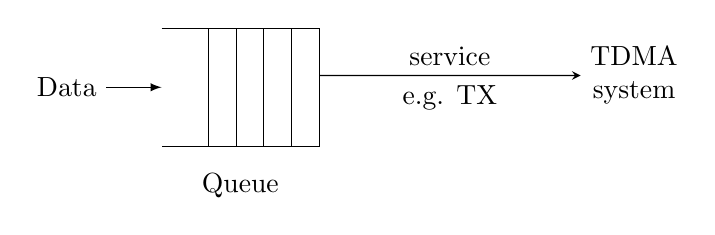
\begin{tikzpicture}[>=latex]
% the rectangle with vertical rules
\draw (0,0) -- ++(2cm,0) -- ++(0,-1.5cm) -- ++(-2cm,0);
\foreach \i in {1,...,4}
  \draw (2cm-\i*10pt,0) -- +(0,-1.5cm);

% the circle
\node[align=center] at (6cm,-0.6) (tdma) {TDMA \\ system};

% the arrows and labels
\path[-stealth] (2cm,-0.6cm) edge[above] node[above]{service} node[below]{e.g. TX}  (tdma);
\draw[<-] (0,-0.75) -- +(-20pt,0) node[left] {Data};
\node[align=center] at (1cm,-2cm) {Queue};
\end{tikzpicture}

% \end{document}
